\section{\ours}
\label{sec:method}

\begin{figure*}[t]
\centering
\resizebox{\textwidth}{!}{% Fig. 2: architecture of the method (schematic in TikZ, v4 2026-10-23). Spec: docs/writing/v2_figure_specs.md (Fig. 2).
% Semantic colors: obscol (observation), predcol (prediction / world), actcol (action), gtcol (neutral).
% The picture is about 17.4 cm wide and is scaled to \textwidth, so \scriptsize prints at about 7 pt.
\begin{tikzpicture}[
  yscale=0.92,
  font=\sffamily\scriptsize,
  >={Stealth[length=4pt,width=3pt]},
  box/.style={draw=gtcol!70, rounded corners=2pt, align=center, inner sep=2.5pt, fill=white, text width=2.85cm},
  lane/.style={rounded corners=2pt, align=left, inner sep=2.5pt, minimum height=0.60cm, text width=3.95cm},
  flowarrow/.style={->, thick, gtcol!80},
  readout/.style={->, thick, predcol, dashed},
]
% ======================= Titles =======================
\node[font=\sffamily\footnotesize\bfseries, anchor=west] at (0,5.12) {Inputs at capture time $\tau_t$};
\node[font=\sffamily\footnotesize\bfseries, anchor=west] at (4.55,5.12) {World--action transformer};
\node[font=\sffamily\footnotesize\bfseries, anchor=west] at (11.75,5.12) {World outputs (training only)};
% ======================= Inputs =======================
\draw[gtcol!70, fill=gtcol!8, rounded corners=1pt] (0.05,3.92) rectangle (1.10,4.80);
\fill[gtcol!25] (0.05,3.92) -- (0.42,4.30) -- (0.70,4.12) -- (1.10,4.50) -- (1.10,3.92) -- cycle;
\fill[obscol] (0.48,4.40) rectangle (0.66,4.56);
\node[box, anchor=west] (img) at (1.22,4.36) {Current RGB-D frame\\frozen \cfgVisualEncoder\\\cfgPatches{} patches + metric XYZ};
\draw[obscol!35, line width=0.6pt] (0.12,2.72) .. controls (0.45,3.37) and (0.75,2.77) .. (1.05,3.30);
\foreach \x/\y/\o in {0.12/2.72/30, 0.42/3.05/50, 0.74/2.97/75, 1.05/3.30/100}{
  \begin{scope}[shift={(\x,\y)}]
    \draw[obscol!\o, line width=0.7pt, ->] (0,0) -- (0.20,0.06);
    \draw[obscol!\o, line width=0.7pt, ->] (0,0) -- (-0.05,0.20);
  \end{scope}}
\node[anchor=north west, text=obscol, inner sep=1pt] at (-0.02,2.45) {$-$\cfgHistorySpan{} to 0};
\node[box, anchor=west, draw=obscol] (hist) at (1.22,3.02) {Target SE(3) history\\\cfgHistoryLen{} steps: pose +\\interval motion};
\node[box, anchor=west] (robot) at (1.22,1.86) {Robot state history\\\cfgHistoryLen{} steps};
% ======================= Transformer =======================
\draw[gtcol!60, rounded corners=4pt, fill=gtcol!4] (4.55,1.27) rectangle (11.35,4.88);
\draw[predcol!70, rounded corners=3pt, fill=predcol!5, dashed] (4.75,2.80) rectangle (9.18,4.84);
\node[anchor=south west, text=predcol!80!black, inner sep=1pt] at (4.80,2.82) {world stream};
\node[lane, fill=obscol!12, draw=obscol] (laneS) at (6.95,4.38) {\textbf{Scene} $\mathcal S$: \cfgPatches{} patch,\\\cfgHistoryLen{} target, \cfgHistoryLen{} robot tokens};
\node[lane, fill=predcol!15, draw=predcol] (laneM) at (6.95,3.48) {\textbf{Summary} $\mathcal M$: \cfgMetaTokens{}\\learnable tokens};
\node[lane, fill=actcol!12, draw=actcol] (laneA) at (6.95,1.90) {\textbf{Action} $\mathcal A$: \cfgChunk{} commands,\\conditional flow matching};
\node[align=center, text=gtcol, text width=2.05cm] at (10.35,2.45) {shared attention,\\stream FFNs\\($\times$\cfgLayers)};
\draw[->, thick, gtcol!70] (laneS.south) -- (laneM.north);
\draw[->, thick, actcol] (laneM.south) -- node[right, text=actcol!80!black, align=left] {reads summary\\tokens only} (laneA.north);
% input arrows
\draw[flowarrow] (img.east) -- (laneS.west |- img.east);
\draw[flowarrow] (hist.east) -- ++(0.18,0) |- ([yshift=-3pt]laneS.west);
\draw[flowarrow] (robot.east) -- ++(0.30,0) |- ([yshift=-8pt]laneS.west);
% ======================= Outputs =======================
\draw[predcol!60, line width=0.6pt] (11.85,3.92) .. controls (12.65,4.72) and (13.30,3.92) .. (14.20,4.57);
\foreach \x/\y/\o in {11.85/3.92/40, 12.40/4.30/55, 12.98/4.24/70, 13.60/4.25/85, 14.20/4.57/100}{
  \begin{scope}[shift={(\x,\y)}]
    \draw[predcol!\o!gtcol, line width=0.8pt, ->] (0,0) -- (0.24,0.05);
    \draw[predcol!\o!gtcol, line width=0.8pt, ->] (0,0) -- (-0.04,0.24);
  \end{scope}}
\node[anchor=west, align=left] at (14.50,4.26) {\textbf{Target SE(3)}\\$(\vect d_h,\boldsymbol\phi_h)$, $h\le\cfgHorizons$};
\foreach \i in {0,...,4}{\foreach \j in {0,...,2}{
  \pgfmathsetmacro{\dx}{0.18+0.05*\j}
  \draw[predcol!70, ->, line width=0.55pt] ({11.90+0.50*\i},{2.62+0.27*\j}) -- ++(\dx,{0.06*\i-0.08});}}
\node[anchor=west, align=left] at (14.50,3.05) {\textbf{Sparse 3D flow}\\$F_h$ + visibility, \cfgContextGrid\\\textcolor{gtcol}{+ depth, DINO, RGB}};
\draw[readout] (9.18,4.22) -- (11.72,4.22);
\draw[readout] (9.18,3.30) -- (11.24,3.30) |- (11.72,2.86);
\node[anchor=south, text=predcol!80!black] at (10.45,4.22) {readout heads};
% attention mask (rows read columns): S, M, A
\def\mx{12.30}\def\my{1.12}\def\cs{0.30}
\foreach \r/\rn in {0/S,1/M,2/A}{
  \node[anchor=east] at (\mx-0.03,{\my+(2-\r)*\cs+0.5*\cs}) {$\mathcal{\rn}$};
  \node[anchor=south] at ({\mx+\r*\cs+0.5*\cs},{\my+3*\cs-0.04}) {$\mathcal{\rn}$};}
\foreach \r/\c/\col in {0/0/obscol, 1/0/predcol, 1/1/predcol, 2/1/actcol, 2/2/actcol}{
  \fill[\col!45] ({\mx+\c*\cs},{\my+(2-\r)*\cs}) rectangle ++(\cs,\cs);}
\draw[gtcol!80, shift={(\mx,\my)}] (0,0) grid[step=\cs] ({3*\cs},{3*\cs});
\node[anchor=west, align=left] at ({\mx+3*\cs+0.18},{\my+1.5*\cs}) {attention mask $\mathcal G$\\(row reads column)};
% ======================= Physical time =======================
% 1.25 cm per 50 ms; capture at x = 5.00, first execution at x = 7.00 (latency 80 ms in this sketch).
\fill[actcol!14] (7.00,0.43) rectangle (8.25,0.67);
\draw[->, gtcol] (4.55,0.55) -- (17.35,0.55);
\node[anchor=north east, text=gtcol] at (17.35,0.47) {physical time};
\draw[gtcol, line width=0.8pt] (5.00,0.42) -- (5.00,0.70);
\node[anchor=north] at (5.00,0.40) {$\tau_t$};
\foreach \h in {1,...,8}{\draw[predcol, line width=0.7pt] ({5.0+1.25*\h},0.48) -- ({5.0+1.25*\h},0.62);}
\node[anchor=north, text=actcol!75!black] at (7.62,0.40) {executed};
\node[anchor=north, text=predcol] at (12.30,0.40) {forecast horizons $\tau_t+\delta_h$, $\delta_h=h\cdot$\cfgHorizonStep};
\foreach \k in {0,...,7}{
  \pgfmathtruncatemacro{\shade}{\k<1 ? 85 : 30}
  \fill[actcol!\shade] ({6.86+1.25*\k},0.70) rectangle ++(0.28,0.26);}
\draw[<->, actcol] (5.00,0.83) -- (6.80,0.83) node[midway, above=-1pt] {latency $\ell_t$};
\node[anchor=west, text=actcol] at (16.02,0.83) {$\tapp_{t,j}$};
\draw[flowarrow, actcol] (laneA.east) -- (9.60,1.90) -- (9.60,1.10) -| (7.00,0.99);
% replan loop
\draw[->, dashed, gtcol!80] (8.25,0.43) -- (8.25,-0.05) -- (0.25,-0.05) -- (0.25,1.52);
\node[anchor=south west, text=gtcol] at (0.40,-0.04) {execute $\to$ observe $\to$ replan};
\end{tikzpicture}
}
\caption{\textbf{\ours。}条件 token $\mathcal Z$ 编码当前 RGB-D 帧、因果跟踪器给出的目标 SE(3) 历史以及机器人状态。物体查询 $\mathcal Q$ 与场景查询 $\mathcal F$ 在物理时域 $\tau_t+\delta_h$ 上回归目标的 SE(3) 轨迹以及带可见性的\QtwoSel{粗粒度}{粗粒度}{\cfgContextPoints{} 个点的} 3D 场景流，外观读出头提供额外的训练目标。动作 token $\mathcal A$ 生成以领先时长为条件、在 $\tapp_{t,j}$ 生效的指令，每 \cfgReplan{} 重规划一次。掩码 $\mathcal G$ 规定每个组读取哪些组。
\QthreeSel{动作 token 在每一层读取世界查询。}{动作 token 读取解码出的世界几何。}{动作 token 不读取任何世界 token，因此部署时只运行动作分支。}}
\label{fig:architecture}
\end{figure*}

\ours（图~\ref{fig:architecture}）是一个包含三组 token 的 Transformer：条件 token 编码当前观测与目标的运动历史，世界查询在物理时域上预测场景，动作 token 生成以领先时长为条件的指令。我们以确定性方式预测世界，用流匹配生成动作 \cite{flowmatching}。下面先说明促成这一设计的问题设定。

\subsection{在物理时间中行动}
\label{sec:formulation}

\paragraph{生效时刻。}
我们考虑一个连同采集时刻一起接收图像与机器人状态的策略。在查询 $t$，其历史为 $\mathcal H_t=\{(o_i,s_i,\tau_i)\}_{\tau_i\le\tau_t}$，输出一个动作块 $A_t=(\vect a_{t,0},\ldots,\vect a_{t,H-1})$，其中第 $j$ 条指令在
\begin{equation}
\tapp_{t,j}=\tau_t+\ell_t+j\Delta_a
\label{eq:apptime}
\end{equation}
生效，$\ell_t$ 是从采集到首次生效的延迟（预处理、推理、排队与执行），$\Delta_a$ 是控制周期。我们把 $\Delta_{t,j}=\tapp_{t,j}-\tau_t$ 称为指令 $j$ 的\emph{领先时长}；这条指令必须与 $\tapp_{t,j}$ 而不是 $\tau_t$ 时的场景相符（图~\ref{fig:principles}）。

\begin{figure}[t]
\centering
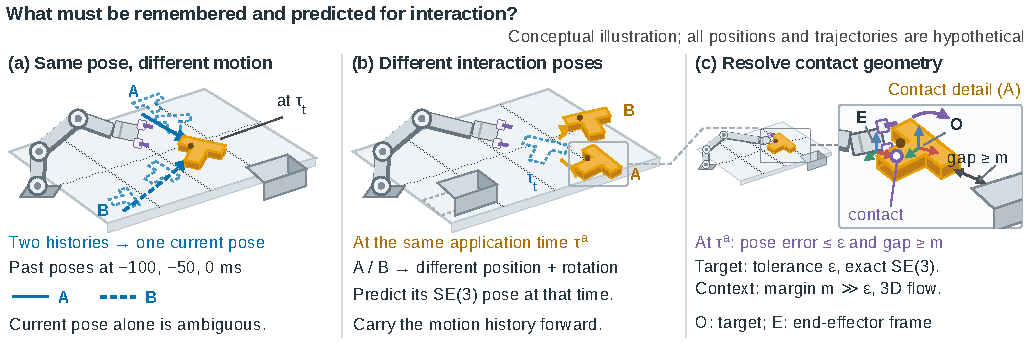
\includegraphics[width=\columnwidth,trim=0 0 0 26,clip]{interaction_timing.pdf}
\caption{\textbf{在物理时间中行动}（示意）。(a) 两段历史在采集时刻 $\tau_t$ 到达同一位姿，却意味着不同的运动。(b) 在生效时刻 $\tapp$，它们导致不同的目标位姿。(c) 接触要求末端坐标系 $E$ 与目标 $O$ 在 $\varepsilon$ 内对齐，而环境只通过它留下的间隙起作用，$m\gg\varepsilon$。}
\label{fig:principles}
\end{figure}

\paragraph{目标与环境。}
令 $W_t(\vect x,\tau)\in\R^3$ 为位于 $\vect x$ 的场景点在 $\tau_t$ 与 $\tau$ 之间的位移，在机器人基座坐标系中表示。\emph{目标} $\mathcal O$ 是其位姿误差进入接触或容纳容差 $\varepsilon$ 的刚体，例如要抓取的物体或要放入的料箱。\emph{环境} $\mathcal C$ 包含只需以间隙 $m$ 避开的物体——传送带或遮挡物。同一物体可以同时扮演两种角色，例如入口必须精确对准、环路必须避开的导线。在目标上，运动场由其位姿 $T(\tau)=(R(\tau),\vect p(\tau))\in\mathrm{SE}(3)$ 决定：
\begin{equation}
W_t(\vect x,\tau)=T(\tau)\,T(\tau_t)^{-1}\vect x-\vect x,\qquad \vect x\in\mathcal O .
\label{eq:rigidfield}
\end{equation}

\paragraph{误差从何而来。}
设策略显式或隐式地依据目标在 $\tapp$ 时位姿的估计 $\hat T$ 行动。对力臂为 $r$ 的接触点与旋转误差 $\theta$，接触误差至多为 $\|\hat{\vect p}(\tapp)-\vect p(\tapp)\|+2r\sin(\theta/2)$。把领先时长 $\Delta$ 内的运动写成匀速 $\vect v$ 加残差 $\boldsymbol\rho$（加速度、滚动、撞击），得到
\begin{equation}
\|\hat{\vect p}(\tapp)-\vect p(\tapp)\|\le
e_{\rm loc}+\hat\Delta\,e_{v}+\|\vect v\|\,e_{\tau}+e_{\rm dyn},
\label{eq:budget}
\end{equation}
四项依次为当前位置误差、速度误差乘领先时长、时间误差乘速度，以及残差运动的误差（附录~\appref{app:analysis}）。对于环境，只有当沿指令路径某处的预测误差至少为 $m$ 时才会发生碰撞。因此，忽略运动的策略一旦 $\|\vect v\|\Delta$ 超过 $\varepsilon$ 就会失手，而环境可以预测得粗得多。这些观察促成了 \ours 的三个部分，当前位置（$e_{\rm loc}$）则依赖位姿跟踪器：度量的运动历史，针对速度误差 $e_v$（第~\ref{sec:remember}~节）；目标的 SE(3) 预测加粗粒度环境流，针对 $e_{\rm dyn}$ 与旋转误差（第~\ref{sec:predict}~节）；知道自身领先时长、并与生效时刻的预测一起训练的指令，针对 $e_\tau$（第~\ref{sec:act}~节）。

\subsection{度量的目标运动历史}
\label{sec:remember}
我们用因果跟踪器在每个全分辨率 RGB-D 帧中估计目标位姿。SAM~2 从目标上的提示出发传播掩码 \cite{sam2}，FoundationPose 依据 CAD 模型或少量参考视图跟踪物体 \cite{foundationpose}。两者都没有时，我们使用逐帧估计度量包围盒位姿的单目三维检测器 \cite{wilddet3d}。每个估计只输出一次，带有其采集时刻与有效标志，之后的帧不会修改它。我们在 $-350,-300,\ldots,0$\,ms 处对这条因果轨迹重采样，使其含义不依赖于相机频率，并构建 \cfgHistoryLen{} 个运动 token，包含区间运动、有限差分速度与加速度以及当前位姿，均在基座坐标系与物理单位下表示（附录~\appref{app:tokens}）。冻结的 \cfgVisualEncoder{} \cite{mae} 把当前 RGB 图像编码为 \cfgPatches{} 个图像块 token，深度图为每个图像块提供用于旋转位置注意力的度量 3D 位置。机器人 token 保存 \cfgHistoryLen{} 个末端状态以及为第一个生效时刻指令的位姿。模型不接收过去的图像；训练时它使用与测试时相同的因果位姿估计，包括跟踪失败。

\subsection{按角色划分的 4D 预测}
\label{sec:predict}
世界查询在时域 $\tau_t+\delta_h$ 上预测 $W_t$，其中 $\delta_h=h\cdot$\cfgHorizonStep{}，$h=1,\ldots,\cfgHorizons$，覆盖下一次重规划之前所执行指令的领先时长，使预测在指令生效的时刻受到监督（附录~\appref{app:budget_leads}）。目标通过式~\eqref{eq:rigidfield} 参数化。对每个时域，
\begin{equation}
\vect d_h=\vect p(\tau_t{+}\delta_h)-\vect p(\tau_t),\;\;
\boldsymbol\phi_h=\Log\!\big(R(\tau_t{+}\delta_h)R(\tau_t)^{\!\top}\big)^{\vee}.
\label{eq:poselabel}
\end{equation}
物体查询以平方平移误差加 $\lambda_R$ 倍平方测地旋转误差回归 $(\vect d_h,\boldsymbol\phi_h)$（$\mathcal L_P$）。对旋转对称的目标，我们排除绕对称轴的不可观测旋转。场景的其余部分表示为 3D 场景流，即固定 \cfgContextGrid{} 图像网格上 $N=\cfgContextPoints$ 个点在基座坐标系中的位移 $F_h\in\R^{N\times3}$，这些点在工作空间中相距约 \fillin{X}\,mm。每个点对应一个带角色嵌入（目标、机器人或环境）的场景查询，回归该点的位移与可见性（$\mathcal L_F$）。\QtwoSel{网格刻意取得较粗，因为环境的误差在其间隙之内都可以容忍。}{网格刻意取得较粗，因为环境的误差在其间隙之内都可以容忍。}{其分辨率是在我们基准中最窄间隙处仍能保持成功率的最粗网格。}未来深度、DINOv3 特征 \cite{dinov3} 与运动表面的 RGB 作为场景查询的额外训练目标（$\mathcal L_{\rm aux}$）。所有标签都从当前状态累计，损失只使用有效标签。

\subsection{以领先时长为条件的动作}
\label{sec:act}
一个动作块包含 \cfgChunk{} 条按式~\eqref{eq:apptime} 的时刻生效的指令，控制周期 $\Delta_a$ 为 50\,ms（\cfgControlRate{}）。每 \cfgReplan{} 重规划一次时，动作块的前两条指令会在下一个动作块替换其余指令之前执行。每条指令是末端在基座坐标系中的平移与左乘相对旋转，外加一个夹爪指令，以为前一个生效时刻所指令的位姿为参考，这一位姿控制器确切知道 \cite{vlash}。每个动作 token 嵌入其领先时长 $\Delta_{t,j}=\ell_t+j\Delta_a$。训练时我们采样 $\ell\sim\mathcal U[0,\cfgLatencyMax]$，并从示范的 $\tau_t+\ell+j\Delta_a$ 处读取指令标签，因此一个模型可服务于该范围内的任何延迟。对归一化的动作块 $\vect a_1$、噪声 $\vect a_0\sim\mathcal N(0,I)$ 与 $u\sim\mathcal U[0,1]$，动作损失为
\begin{equation}
\mathcal L_A=\mathbb E\,\big\|v_\psi(\vect a_u,u\mid\mathcal Z_t,\hat{\mathcal W}_t,\mathcal G)-(\vect a_1-\vect a_0)\big\|^2,
\label{eq:fm}
\end{equation}
其中 $\vect a_u=(1-u)\vect a_0+u\vect a_1$，$\mathcal Z_t$ 为条件 token，$\hat{\mathcal W}_t$ 为耦合方式允许动作读取的世界 token（R0 与 R1 中没有）。总损失为 $\mathcal L=\mathcal L_A+\lambda_F\mathcal L_F+\lambda_P\mathcal L_P+\lambda_{\rm aux}\mathcal L_{\rm aux}$。

\paragraph{世界—动作耦合。}
注意力掩码 $\mathcal G$ 作用于四个 token 组：条件 $\mathcal Z$、物体查询 $\mathcal Q$、场景查询 $\mathcal F$ 与动作 $\mathcal A$。条件 token 只相互读取；世界查询读取条件与彼此；动作 token 读取条件、自身以及耦合方式所允许的那部分世界。
\Qthree{1}{动作 token 在每一层读取 $\mathcal Q$ 与 $\mathcal F$ 的隐藏状态，而世界不读取动作。}%
\Qthree{2}{我们每次查询预测一次世界，把解码出的目标轨迹与场景流编码为几何条件 token，并由它们以 \cfgEuler{} 步欧拉积分生成动作。训练时梯度穿过预测的几何反向传播，不使用教师强制。}%
\Qthree{3}{动作不读取任何世界 token。世界损失在训练中塑造共享参数，部署时只运行动作分支。}
\Bbone{1}{两个分支共享注意力投影，各自拥有前馈网络。}%
\Bbone{2}{世界分支与动作分支参数分离，条件 token 经过世界组，因此世界监督也塑造动作所读取的内容。}
第~\ref{sec:principles}~节把这一选择与其他方案进行比较，记号如下：R0 关闭世界损失，R1 中动作不读取任何世界 token，R2 中动作读取世界查询的隐藏状态，R3 中世界读取带噪动作，R4 双向开放，R5 把解码出的几何编码后供动作读取（附录~\appref{app:coupling}）。

\paragraph{执行与实现。}
测试时，我们依据执行器的延迟估计设定领先时长，即近期推理时间的 p95 加执行延迟。Transformer 有 \cfgLayers{} 层、宽度 \cfgWidth{}、\cfgHeads{} 个头，主干参数 \cfgBackboneParams{}，可训练参数共 \cfgTrainableParams{}。图像编码器与 DINOv3 教师保持冻结，但在每个训练步都要运行，并占据了其主要开销。在 \bench 上，我们以数据并行训练 4 个 epoch（全局 batch 为 16 时约 40k 次更新），在 \cfgTrainHardwareZh{} 上每个训练种子约需 \cfgTrainHours{} 小时。测试时，动作分支以半精度进行 \cfgEuler{} 步欧拉积分，在一块 \cfgGPU{} 上的 p95 出动作时间为 \fillin{XX}\,ms（附录~\appref{app:recipe} 与附录~\appref{app:timing}）。

\subsection{在提升为 4D 的真实机器人数据上预训练}
\label{sec:pretraining}
真实机器人数据不提供物体位姿或场景流。我们不使用物体模型，将 DROID \cite{droid} 提升为度量 4D 标签。场景流来自 PointWorld 为 DROID 发布的 3D 轨迹与优化后的相机标定 \cite{pointworld}。我们把指令中提到的物体作为目标：开放词汇检测器找到它 \cite{groundingdino}，SAM~2 跟踪其掩码，单目三维检测器估计其度量位姿。输入来自前向跟踪，与部署时一致；式~\eqref{eq:poselabel} 的标签来自整段回合上平滑的前向—后向跟踪。DROID 中的目标大多在机器人移动它们时才运动（\fillin{X}\% 的窗口在接触前出现目标运动），因此预训练主要教会模型度量几何、3D 流以及它们与以领先时长为条件的动作之间的耦合（图~\appref{fig:lifting}）。真机策略从这一基座初始化。仿真模型从通用初始化（冻结的 MAE 编码器加随机初始化的 Transformer）训练，另有一组受控比较在 \bench 上对基座做后训练（附录~\appref{app:pretraining}）。
